\chapter{Getting to understand Ultra Orthogonality in the $XY$ Model.}

As discussed in the previous chapters, we are interested in solvable Fermionic systems. Indeed the one dimensional $XY$ model is one of those systems\cite{lieb_two_1961}. The XY Hamiltonian model is a set of $N$ spin $1/2$ particles 
located on the sites of d-dimensional lattice. Nevertheless, whenever we talk about the $XY$ model, we will be referring to the $1D$ $XY$ model.
\section{The $XY$ Model}
A chain of $N$ spins where each spin is able to interact with its nearest neighbours in the $X$ and $Y$ coordinate as well as an external magnetic field, will be described by the Hamiltonian of the form
\begin{equation}
H_{X Y}=-\frac{1}{2} \sum_{l=0}^{N-1}\left(\frac{1+\gamma}{2} \sigma_{l}^{x} \sigma_{l+1}^{x}+\frac{1-\gamma}{2} \sigma_{l}^{y} \sigma_{l+1}^{y}+\lambda \sigma_{l}^{z}\right),
\label{CH3:Hamiltonian_XY}
\end{equation}
where $\gamma$ is so-called the anisotropy parameter and represents the difference between the strength of the $XX$ interaction and the $YY$ interaction\footnote{When we talk about interactions we mean interactions between spins.}, $\lambda$ is the intensity of the external magnetic field and $\sigma^{i}_{l}$ is the Pauli matrix ($i= x,y,z$) acting over the $l$ site of the chain.\\
The XY model is a model that has been widely studied for a variety of values of $\lambda$ and $\gamma$ and in some limits it has a correspondence to other models of interest in condensed matter\cite{katsura_statistical_1962,barouch_statistical_1971,barouch_statistical_1970}\footnote{Some examples of this kind, are the boson Hubbard model in the limit of hard bosons. the case when $\gamma=1$ correspond to the Ising model, and the Kitaev chain is equivalent to the XY model under a proper identification of the parameters $\mu$, $t$ and $\Delta$ with $\gamma$ and $\lambda$\cite{katsura_statistical_1962,barouch_statistical_1971}}.
\subsection{The spectrum}
To find the spectrum of the Hamiltonian \eqref{CH3:Hamiltonian_XY} we need to perform some special transformations.
\subsection{Jordan-Wigner Transformation}
We first consider the non local transformation given by
\begin{equation}
\hat{b}_{l}=\left(\prod_{m<l} \sigma_{m}^{z}\right) \sigma_{l}^{-}, \quad \sigma_{l}^{-}=\frac{\sigma_{l}^{x}-i \sigma_{l}^{y}}{2},
\end{equation}
where these $b_l$ represent spinless Fermionic operators, and its canonical anticommutation relation (CAR) is given by\cite{reyes-lega_aspects_2016} 
\begin{equation}
\left\{\hat{b}_{i}^{\dagger}, \hat{b}_{j}^{\dagger}\right\}=\left\{\hat{b}_{i}, \hat{b}_{j}\right\}=0, \quad\left\{\hat{b}_{i}^{\dagger}, \hat{b}_{j}\right\}=\delta_{i, j}.
\end{equation}
So inverting the transformation we get 
\begin{equation}
\begin{array}{l}
\sigma_{l}^{z}=1-2 \hat{b}_{l}^{\dagger} \hat{b}_{l} \\
\sigma_{l}^{x}=\left(\prod_{m<l}\left(1-2 \hat{b}_{m}^{\dagger} \hat{b}_{m}\right)\right)\left(\hat{b}_{l}^{\dagger}+\hat{b}_{l}\right) \\
\sigma_{l}^{y}=i\left(\prod_{m<l}\left(1-2 \hat{b}_{m}^{\dagger} \hat{b}_{m}\right)\right)\left(\hat{b}_{l}^{\dagger}-\hat{b}_{l}\right).
\end{array}
\end{equation}

The terms of interaction in the Hamiltonian will look as
\begin{equation}
\begin{aligned}
\hat{\sigma}_{l}^{x} \hat{\sigma}_{l+1}^{x} &=\left(\hat{b}_{l}^{\dagger}-\hat{b}_{l}\right)\left(\hat{b}_{l+1}^{\dagger}+\hat{b}_{l+1}\right) \\
\hat{\sigma}_{l}^{y} \hat{\sigma}_{l+1}^{y} &=-\left(\hat{b}_{l}^{\dagger}+\hat{b}_{l}\right)\left(\hat{b}_{l+1}^{\dagger}-\hat{b}_{l+1}\right)
\end{aligned},
\end{equation}
and the Hamiltonian will look like,
\begin{equation}
H_{X Y}=-\frac{1}{2} \sum_{l}\left[\left(\hat{b}_{l+1}^{\dagger} \hat{b}_{l}+\hat{b}_{l}^{\dagger} \hat{b}_{l+1}\right)+\gamma\left(\hat{b}_{l}^{\dagger} \hat{b}_{l+1}^{\dagger}-\hat{b}_{l} \hat{b}_{l+1}\right)\right]-\frac{\lambda}{2} \sum_{l}\left(1-2 \hat{b}_{l}^{\dagger} \hat{b}_{l}\right),
\end{equation}
after this transformation. The term of $-\lambda N/2$ is usually ignored since it cause only a gauge of the spectrum in the energy\cite{reyes-lega_aspects_2016} .
\subsection{Fourier Transformation}
It is possible to exploit an other symmetry in the system. It comes by considering periodic boundary conditions (PBC)\cite{reyes-lega_aspects_2016} . This can be easily done by identifying the spin in the site $N$ with the spin in the site $1$. After imposing this condition, we have that the Fourier transform of the operator $\hat{b}_l$ will look as
\begin{equation}
\hat{d}_{k}=\frac{1}{\sqrt{N}} \sum_{l=1}^{N} \hat{b}_{l} e^{-i \phi_{k} l},
\end{equation}
with $\theta_{k}=\frac{2 \pi}{N} k$.\\
Since the Fourier transformation is unitary, the operators $\hat{d}_k$ will preserve the CAR.
\begin{figure}[H]
    \centering
    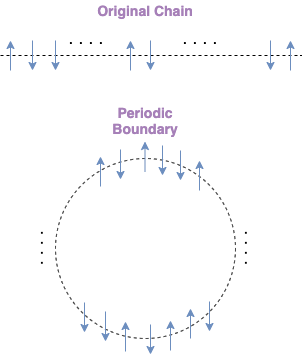
\includegraphics[width=0.4\textwidth]{Figures/Periodic_boundaries.png}
    \caption{Illustration of what a boundary condition means in the case of our spin chain}
    \label{periodic condition}
\end{figure}
Thus, the Hamiltonian can be written in terms of the operators $\hat{d}_k$ as
\begin{equation}
H_{X Y}=\sum_{k=-(N-1) / 2}^{(N-1) / 2}\left(-\lambda+\cos \phi_{k}\right) \hat{d}_{k}^{\dagger} \hat{d}_{k}+\frac{i \gamma}{2} \sum_{k=-(N-1) / 2}^{(N-1) / 2} \sin \phi_{k}\left(\hat{d}_{k} \hat{d}_{-k}+h . c\right),
\end{equation}
where we have ignored an additional term which is proportional to $1/N$ which will vanish for in the thermodynamic limit $N\to \infty$\cite{barouch_statistical_1970,barouch_statistical_1971}, which is our case of interest.
\subsection{Bogoliubov -Valantin Transformation}
As mentioned before Fermionic quadratic Hamiltonians can be easily diagonalised via a Bogoliubov-Valantin transformation over the operators $\hat{d}_k$

\begin{equation}
\tilde{d}_{k}=u_{k} \hat{d}_{k}^{\dagger}+i v_{k} \hat{d}_{-k}.
\end{equation}
Since we want this transformation to preserve CAR, it is needed that $u_k^2 + v_k^2 = 1$, which implies that we can use the parametrization $u_{k}=\cos \left(\psi_{k} / 2\right)$ and $v_{k}=\sin \left(\psi_{k} / 2\right)$, with
\begin{equation}
\cos \frac{\psi_{k}}{2}=\frac{-\lambda+\cos \phi_{k}}{\sqrt{\left(\lambda-\cos \phi_{k}\right)^{2}+\left(\gamma \sin \phi_{k}\right)^{2}}}
\end{equation}
So finally our Hamiltonian will look as
\begin{equation}
H_{X Y}=\sum_{-(N-1) / 2}^{(N-1) / 2} \tilde{\Lambda}_{k} \tilde{d}_{k}^{\dagger} \tilde{d}_{k}
\end{equation}
with 
\begin{equation}
\tilde{\Lambda}_{k}:=\sqrt{\left(\lambda-\cos \phi_{k}\right)^{2}+\left(\gamma \sin \phi_{k}\right)^{2}}
\label{CH3:Spectrum_XY_model}
\end{equation}
where the latter expression allow us to identify the critical regions of the model.
\subsection{Fermionic Covariance Matrix for the XY model}

As we mentioned before, sometimes it turns out to be better, and useful to work directly with the Covariance matrix. To be able to do so,we need to express the Hamiltonian \eqref{CH3:Hamiltonian_XY} in terms of Majoranana fermions. This can be done by using an analogous of the Jordan Wigner transformation use to diagonalised the XY Hamiltonian but now we apply it to the $2N$ Majorana fermions

\begin{equation}
\hat{\gamma}_{l}=\left(\prod_{m<l} \hat{\sigma}_{m}^{z}\right) \hat{\sigma}_{l}^{x}, \quad \hat{\gamma}_{l+N}=\left(\prod_{m<l} \hat{\sigma}_{m}^{z}\right) \hat{\sigma}_{l}^{y},
\end{equation}
where again $l=1,2\ldots N-1$
\begin{figure}[H]
    \centering
    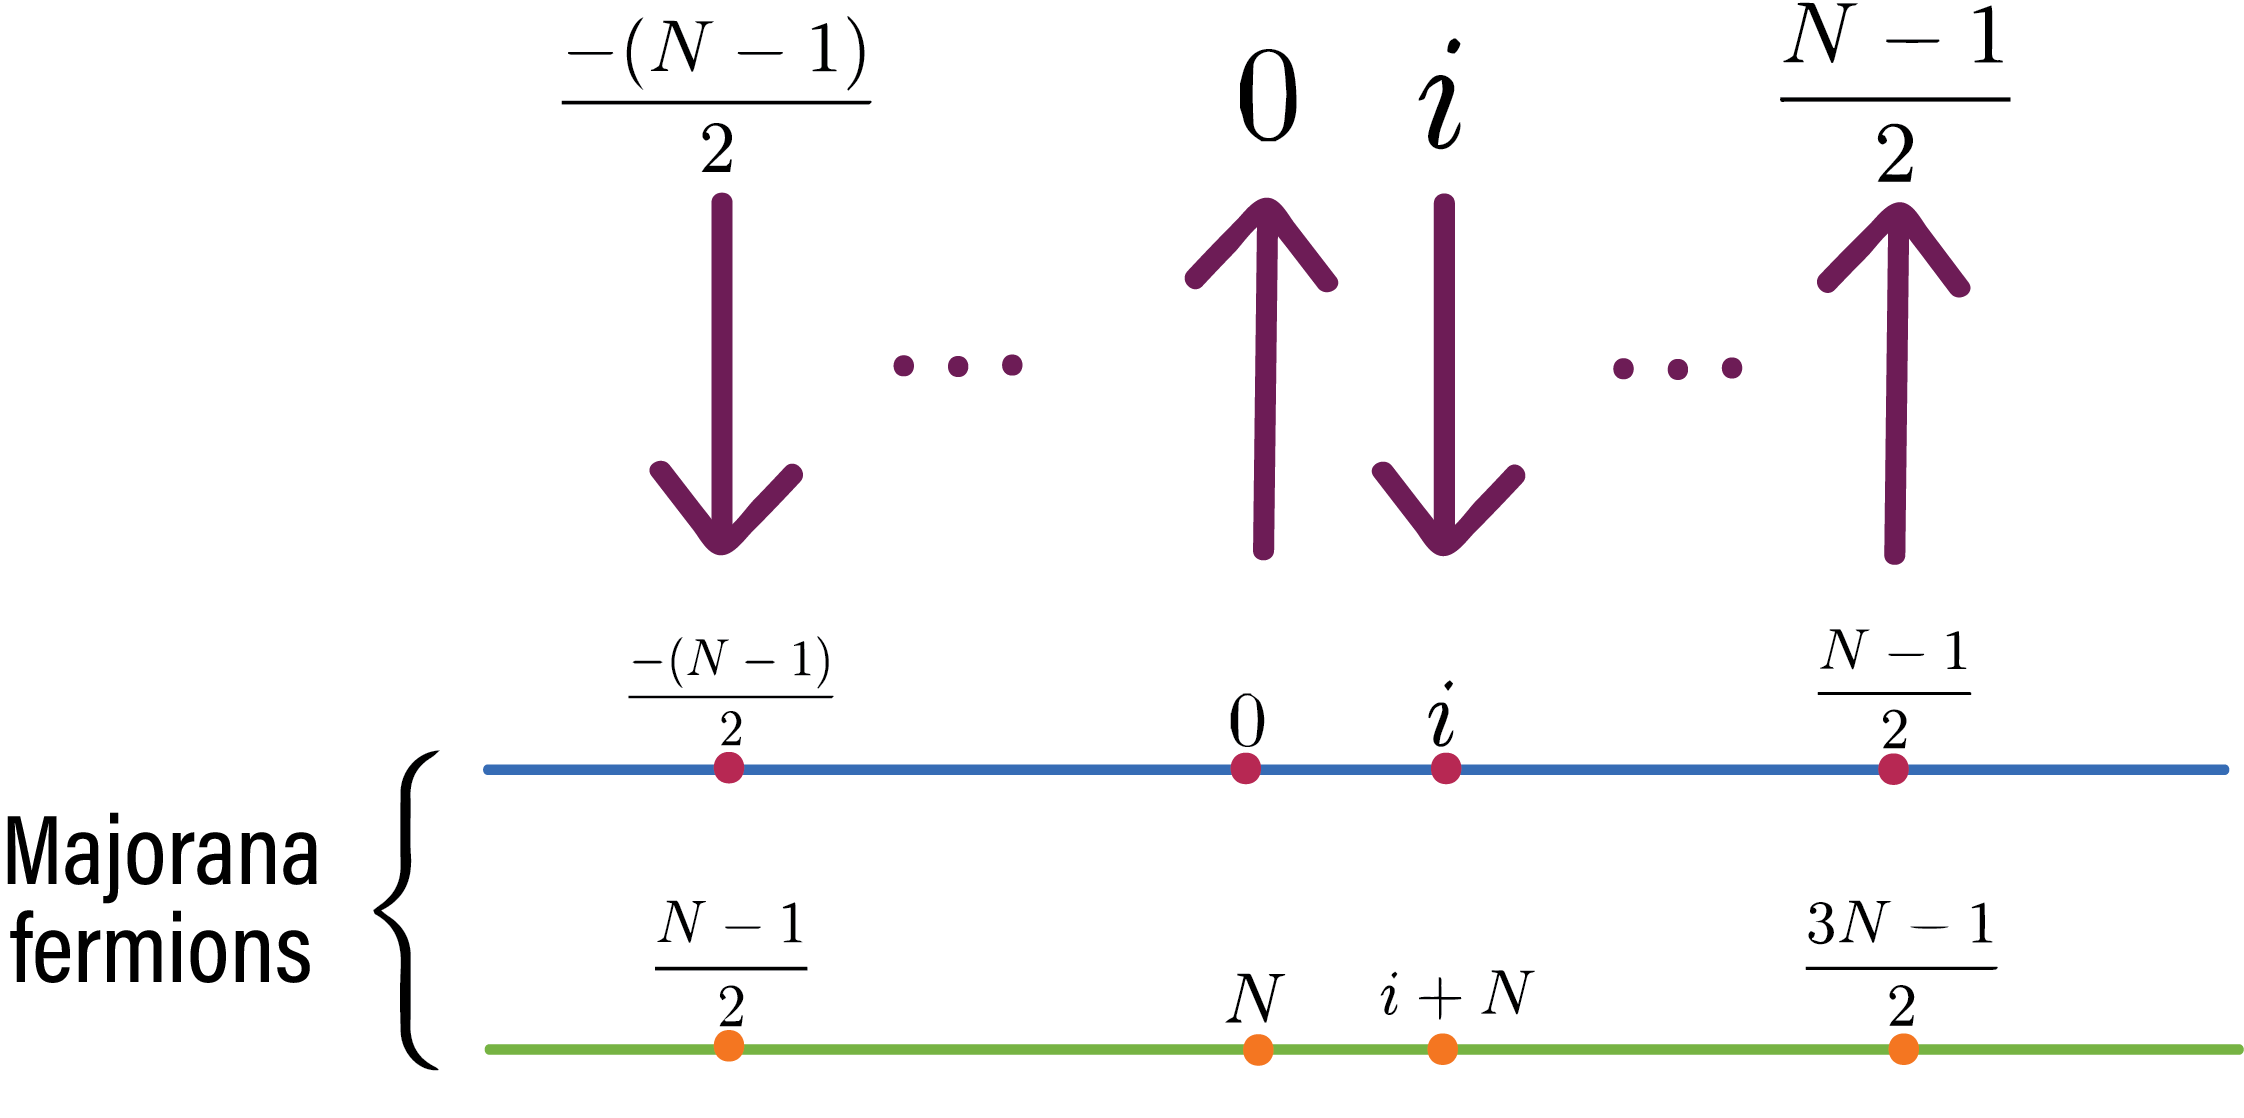
\includegraphics[width=0.5\textwidth]{Figures/ecuacion.png}
    \caption{Illustration of how the spins in the chain are mapped to the Majorana fermions.}
    \label{majorana fermions}
\end{figure}
and similarly as before we have that
\begin{equation}
\hat{\gamma}_{l} \hat{\gamma}_{l+N}=\left(\prod_{m<l} \hat{\sigma}_{m}^{z}\right)\left(\prod_{m<l} \hat{\sigma}_{m}^{z}\right) \hat{\sigma}_{l}^{x} \hat{\sigma}_{l}^{y}=i \hat{\sigma}_{l}^{z},
\end{equation}
\begin{equation}
\hat{\gamma}_{l+N} \hat{\gamma}_{l+1}=\left(\prod_{m<l} \hat{\sigma}_{m}^{z}\right) \hat{\sigma}_{l}^{y}\left(\prod_{m<l+1} \hat{\sigma}_{m}^{z}\right) \hat{\sigma}_{l+1}^{x}=\hat{\sigma}_{l}^{y} \hat{\sigma}_{l}^{z} \hat{\sigma}_{l+1}^{x}=i \hat{\sigma}_{l}^{x} \hat{\sigma}_{l+1}^{x},
\end{equation}
\begin{equation}
\hat{\gamma}_{l} \hat{\gamma}_{l+N+1}=\left(\prod_{m<l} \hat{\sigma}_{m}^{z}\right) \hat{\sigma}_{l}^{x}\left(\prod_{m<l+1} \hat{\sigma}_{m}^{z}\right) \hat{\sigma}_{l+1}^{y}=\hat{\sigma}_{l}^{x} \hat{\sigma}_{l}^{z} \hat{\sigma}_{l+1}^{y}=-i \hat{\sigma}_{l}^{y} \hat{\sigma}_{l+1}^{y}.
\end{equation}
Which coincide, up to constant factors, with the three terms in the Hamiltonian \eqref{CH3:Hamiltonian_XY}. This will lead us to a Hamiltonian of the form\cite{botero_bcs-like_2004,latorre_ground_2004}
\begin{equation}
H_{X Y}=\frac{i}{4} \sum_{\alpha, \beta=0}^{2 N} \Omega_{\alpha \beta}\left[\hat{\gamma}_{\alpha}, \hat{\gamma}_{\beta}\right],
\label{CH3:Hamiltonian_to_diagonalise}
\end{equation}
where $\Omega$ is the antisymmetric matrix of the form
\begin{equation}
\Omega=\left[\begin{array}{c|c}
0 & \tilde{\Omega} \\
\hline -\tilde{\Omega}^{T} & 0
\end{array}\right],
\label{CH3:Block_matrix}
\end{equation}
with 
\begin{equation}
\tilde{\Omega}=\begin{pmatrix}
\lambda & \frac{1-\gamma}{2} & 0 &0 &\ldots  &0 &\frac{1+\gamma}{2}\\
\frac{1+\gamma}{2} & \lambda & \frac{1-\gamma}{2} & 0 &\ldots &0 &0\\
0 & \frac{1+\gamma}{2} & \lambda & \frac{1-\gamma}{2} &\ldots &0 &0\\
\vdots& \ddots & \ddots & \ddots & \ldots &  \vdots & \vdots\\
\frac{1-\gamma}{2}&0&0&0&\ldots & \frac{1+\gamma}{2} & \lambda.
\end{pmatrix}.
\label{CH3:Hamiltonian_matrix_XY_model}
\end{equation}
In general \eqref{CH3:Block_matrix} can be diagonalised via an orthogonal transformation $O$\cite{botero_bcs-like_2004,latorre_ground_2004} \footnote{This special relation provide us a way to transform from spacial modes to excitation in the chain, so that we can either excite the chain and see what the spatial modes are or the other way.}
\begin{equation}
    \Omega=O\left[\begin{array}{c|c}
0 & \omega \\
\hline \omega & 0
\end{array}\right] O^T,
\label{CH3:Matrix_decomposed}
\end{equation}
where $O\in O(2N)$.  Writing it in terms of two smaller orthogonal matrices will look as
\begin{equation}
O=\left[\begin{array}{c|c}
O_1 & 0 \\
\hline 0 & O_2
\end{array}\right],
\end{equation}
and $\omega$ is a diagonal matrix of size $N\times N$ which holds excitation numbers $-1/2+n$. By doing the product of matrices in \eqref{CH3:Matrix_decomposed} we can easily see that 
\begin{equation}
    \tilde{\Omega}=O_1 \omega O_2^T,
\end{equation}
which is nothing but the singular value decomposition of the matrix $\tilde{\Omega}$. The latter result tell us that a fast way to construct the matrix $O$, which diagonalise $\Omega$, is to focus on $\tilde{\Omega}$.
\newline
A fact that we can exploit is that , the matrix described in equation \eqref{CH3:Hamiltonian_matrix_XY_model} $\tilde{\Omega}$ is a circulant real matrix, meaning that it can be easily diagonalised by means of a Fourier transform. So we can write
\begin{equation}
\tilde{\Omega}_{m n}=\frac{1}{N} \sum_{\theta_{k} \in(-\pi, \pi)} \omega\left(\theta_{k}\right) e^{\phi\left(\theta_{k}\right)} e^{i(m-n) \theta_{k}}
\label{CH3:circulant_expantion}
\end{equation}
where $\omega\left(\theta_{k}\right)=\omega\left(\theta_{k}\right)^{*}=\omega\left(-\theta_{k}\right), \phi\left(\theta_{k}\right)=-\phi\left(\theta_{k}\right)$ and are given by
\begin{equation}
\omega^{2}\left(\theta_{k}\right):=\left(\lambda-\cos \theta_{k}\right)^{2}+\gamma^{2} \sin ^{2} \theta_{k},
\end{equation}
and
\begin{equation}
\phi\left(\theta_{k}\right):=\arctan \left(\frac{\lambda-\cos \theta_{k}}{-\gamma \sin \theta_{k}}\right).
\end{equation}
So expanding the equation \eqref{CH3:circulant_expantion}, we get
\begin{equation}
\begin{aligned}
\tilde{\Omega}_{m n} &=\frac{1}{N}\left[\omega(0)+(-1)^{m-n} \omega(\pi)+2 \sum_{0<\theta_{k}<\pi} \omega\left(\theta_{k}\right) \cos \left(\theta_{k}(m-n)+\phi\left(\theta_{k}\right)\right)\right] \\
&=\frac{\omega(0)}{N}+(-1)^{m-n} \frac{\omega(\pi)}{N}+\sum_{0<\theta_{k} \leq \pi} \omega\left(\theta_{k}\right)\left(u_{m}^{c}\left(\theta_{k}\right) v_{n}^{c}\left(\theta_{k}\right)+u_{m}^{s}\left(\theta_{k}\right) v_{n}^{s}\left(\theta_{k}\right)\right),
\end{aligned}
\end{equation}

where
\begin{equation}
u_{m}^{c}\left(\theta_{k}\right)=\sqrt{\frac{2}{N}} \cos \left(m \theta_{k}+\phi\left(\theta_{k}\right)\right), \quad u_{m}^{s}\left(\theta_{k}\right)=\sqrt{\frac{2}{N}} \sin \left(m \theta_{k}+\phi\left(\theta_{k}\right)\right),
\end{equation}
\begin{equation}
v_{n}^{c}\left(\theta_{k}\right)=\sqrt{\frac{2}{N}} \cos \left(n \theta_{k}\right), \quad u_{n}^{s}\left(\theta_{k}\right)=\sqrt{\frac{2}{N}} \sin \left(n \theta_{k}\right).
\end{equation}
Now defining $
u^{s}(0)=v^{s}(\pi)=0 \mathrm{y} u^{c}(0)=v^{c}(\pi)=\frac{1}{\sqrt{N}}$, we have that $\tilde{\Omega}_{m,n}$ can be written as
\begin{equation}
\tilde{\Omega}_{m n}=\sum \omega\left(\theta_{k}\right)\left(u_{m}^{c}\left(\theta_{k}\right) v_{n}^{c}\left(\theta_{k}\right)+u_{m}^{s}\left(\theta_{k}\right) v_{n}^{s}\left(\theta_{k}\right)\right).
\end{equation}
Therefore the upper part of the Hamiltonian reads
\begin{equation}
H=\sum_{m, n=0}^{N-1} \frac{i}{4} \sum_{\theta_{k}=0}^{\pi} \omega\left(\theta_{k}\right)\left(u_{m}^{c}\left(\theta_{k}\right) v_{n}^{c}\left(\theta_{k}\right)+u_{m}^{s}\left(\theta_{k}\right) v_{n}^{s}\left(\theta_{k}\right)\right)\left[\hat{\gamma}_{n}, \hat{\gamma}_{m+N}\right],
\end{equation}

\begin{equation}
H=\sum_{\theta_{k}=0}^{\pi} \omega\left(\theta_{k}\right)(\underbrace{\left[\hat{\gamma}_{k}^{c}, \hat{\gamma}_{k+N}^{c}\right]}_{1-2\sigma^{z     }_k}+\underbrace{\left[\hat{\gamma}_{k}^{s}, \hat{\gamma}_{k+N}^{s}\right]}_{1-2\sigma^{z}_k}),
\end{equation}

where
\begin{equation}
\hat{\gamma}_{k}^{c, s}:=\sum_{n} u_{n}^{c, s}\left(\theta_{k}\right) \hat{\gamma}_{n}, \quad \hat{\gamma}_{k+N}^{c, s}:=\sum_{n} v_{n}^{c, s}\left(\theta_{k}\right) \hat{\gamma}_{n+N}.
\end{equation}
Now we look back on the fact that the Fermionic covariance matrix, defined by $
\Gamma_{\alpha \beta}=\frac{1}{2 i} \operatorname{tr}\left(\rho\left[\gamma_{\alpha}, \gamma_{\beta}\right]\right)=\frac{1}{2 i}\langle \left[\gamma_{\alpha}, \gamma_{\beta}\right] \rangle$, that brings $\Omega$ into its Williamson form, does the same on the Fermionic covariance matrix. Thus for a state $|\vec{n}\rangle$, consider an eigenstate of the base $(c,s,\theta_k)$, where $m^{c, s}\left(\theta_{k}\right)-1 / 2$, with $n^{c, s}\left(\theta_{k}\right)$ the occupation number of \textit{cosine}, \textit{sine} in the $k-$mode. We get 

\begin{equation}
\begin{aligned}
\tilde{\Gamma}_{m n} &=\sum_{\theta_{k}}^{\pi}\left[m^{c}\left(\theta_{k}\right) u_{m}^{c}\left(\theta_{k}\right) v_{n}^{c}\left(\theta_{k}\right)+m^{s}\left(\theta_{k}\right) u_{m}^{s}\left(\theta_{k}\right) v_{n}^{s}\left(\theta_{k}\right)\right] \\
&=\sum_{\theta_{k}}^{\pi}\left(\frac{m^{c}\left(\theta_{k}\right)+m^{s}\left(\theta_{k}\right)}{2}\right)\left(u_{m}^{c}\left(\theta_{k}\right) v_{n}^{c}\left(\theta_{k}\right)+u_{m}^{s}\left(\theta_{k}\right) v_{n}^{s}\left(\theta_{k}\right)\right) \\
&+\sum_{\theta_{k}}^{\pi}\left(\frac{m^{c}\left(\theta_{k}\right)-m^{s}\left(\theta_{k}\right)}{2}\right)\left(u_{m}^{c}\left(\theta_{k}\right) v_{n}^{c}\left(\theta_{k}\right)-u_{m}^{s}\left(\theta_{k}\right) v_{n}^{s}\left(\theta_{k}\right)\right).
\end{aligned}
\end{equation}
by defining $m^{\pm}\left(\theta_{k}\right)=\frac{m^{c}\left(\theta_{k}\right) \pm m^{s}\left(\theta_{k}\right)}{2}$ and inverting the transformations done above, we finally get that
\begin{equation}
\tilde{\Gamma}_{m n}=\overbrace{\sum_{\theta_{k}}^{\pi} m^{+}\left(\theta_{k}\right) e^{i \phi\left(\theta_{k}\right)} e^{i(n-m) \theta_{k}}}^{\tilde{\Gamma}^{+}_{mn}}+\underbrace{\sum_{\theta_{k}}^{\pi} m^{-}\left(\theta_{k}\right) e^{i \phi\left(\theta_{k}\right)} e^{i(n+m) \theta_{k}}}_{\tilde{\Gamma}_{m n}^{-}}.
\end{equation}
We notice that $\tilde{\Gamma}^{+}_{mn}$ is circulant, whereas $\tilde{\Gamma}^{-}_{mn}$ is not, nevertheless, observe that $\tilde{\Gamma}^{+}_{mn} = \tilde{\Gamma}^{}_{mn'}$, with $n'$ a change on the index $n\to -n'$, which can be interpreted as a rotation over the circle.
\begin{figure}[H]
    \centering
    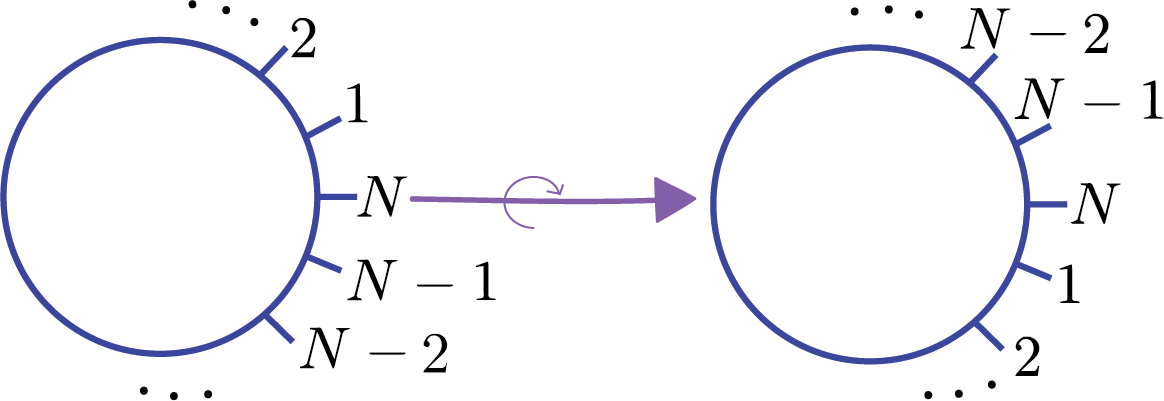
\includegraphics[width=0.6\textwidth]{Figures/Reflection_over_circle.png}
    \caption{Meaning of the relabel done in the circulant matrix, which can be seen as a reflection over the circle.}
    \label{reflectioncircle}
\end{figure}
Explicitly we can write that if $\tilde{\Gamma}^{+}_{mn}$ has the shape
\begin{equation}
\left(\begin{array}{ccccc}
a_{0} & a_{-1} & \cdots & a_{2} & a_{1} \\
a_{1} & a_{0} & \cdots & a_{3} & a_{2} \\
\cdot & \cdot & \cdot & \cdots & \cdot \\
\vdots & \vdots & \vdots & \vdots & \vdots \\
a_{-1} & a_{-2} & a_{-3} & \cdots & a_{0}
\end{array}\right),
\end{equation}
then $\tilde{\Gamma}^{-}_{mn}$ will be given by
\begin{equation}
\left(\begin{array}{ccccc}
a_{0} & a_{1} & \cdots & a_{-2} & a_{-1} \\
a_{1} & a_{2} & \cdots & a_{-1} & a_{0} \\
\cdot & \cdot & \cdot & \cdots & \cdot \\
\vdots & \vdots & \vdots & \vdots & \vdots \\
a_{-1} & a_{0} & a_{1} & \cdots & a_{-2}
\end{array}\right).
\end{equation}

So we can spot 3 things. First, the FCM always can be written as a circulant matrix plus an anticirculant matrix. Second, in the Ground state, the FCM is circulant only, since the fermion occupation numbers $n^{c}\left(\theta_{k}\right)=n^{s}\left(\theta_{k}\right)=0, \forall k$. Third, for a generic state, we have that in average the FCM matrix is always circulant, because $\langle n^{c}\left(\theta_{k}\right)\rangle=\langle n^{s}\left(\theta_{k}\right)\rangle$.\\
Now that we have showed a full characterization of the $XY$ model, we change gears and start to board our problem. In the next section we are going to show how this is possible to find bound for the case of the $XY$ model and we will be able to show that the mechanism for Ultra Orthogonality in this system, is related with the structure of the system.


\section{Exploring ``Ultra Orthogonality''}
Now having all the tools we need we can apply what we discussed in section $2$. First we will look at the error exponents for the $XY$ model, we will compute the probabilities of having errors and show some numerical results. Then we will move to our next problem, we will show for the $XY$ model is possible to bound the determinant and even more we find an analytical result for this determinant based on a generalisation of Szeg\''{o} limit theorems. 

\subsection{Error exponent}

First we recall the fact that in order to sample states at a given temperature we make use of a very well known technique, named Gibbs sampling. This technique is a special case of a Markov chain Monte Carlo algorithm. Is is well known for obtaining sequences of observations which are approximated from a specified multivariate probability distribution, It is a very useful tool for simulations in Markov processes for which the transition from which transition matrix cannot be formulated explicitly because the state space is too large\cite{robert_multi-stage_2004,gilks_markov_1996,noauthor_gibbs_nodate}. Our goal is then to sample over excited states $\ket{\vec{n}}$, where the occupations $n_q$ will be sampled independently according to the Boltzmann distribution
\begin{equation}
p(\vec{n} \mid \beta)=\prod_{q=0}^{N-1} p\left(n_{q} \mid \beta\right), \quad p\left(n_{q} \mid \beta\right)=\frac{e^{-\beta \epsilon\left(\theta_{q}\right) n_{q}}}{\sum_{n_{q}} e^{-\beta \epsilon\left(\theta_{q}\right) n_{q}}},
\label{CH3:Gibbs_Sampling}
\end{equation}
where we explicitly put the dependence of the energy with certain angle in \eqref{CH3:Gibbs_Sampling} having in mind the case of the $XY$ model\footnote{However, the $XY$ model is not the only model in which the energy can be parametrized in terms of an angle, in general it has been shown that every one-dimentional translationally invariant closed chain of free Fermions/Bosons will have this property \cite{eisert_area_2010,fradkin_field_1997,katsura_statistical_1962,latorre_ground_2004,lieb_two_1961}.}. The goal of using this technique  that the size of the Hilbert space is is to find the probability distribution with a given temperature $\beta$. It is well known that in the Fermionic case, the average number of excitations in the mode at angle $\theta$ is given by
\begin{equation}
f\left(\theta_{q} \mid \beta\right) \equiv\left\langle n_{q}\right\rangle_{\beta}=\frac{1}{e^{\beta \epsilon\left(\theta_{q}\right)} + 1},
\end{equation}
while the variance in the number of excitations is given by

\begin{equation}
v\left(\theta_{q} \mid \beta\right) \equiv\left\langle n_{q}^{2}\right\rangle_{\beta}-\left\langle n_{q}\right\rangle_{\beta}^{2}=\frac{1}{e^{\beta \epsilon\left(\theta_{q}\right)} + 1}=f\left(\theta_{q}\right)\left(1 - f\left(\theta_{q}\right)\right).
\end{equation}
With this method of sampling, the mean energy is 
\begin{equation}
\langle E\rangle_{\beta}=\sum_{q} f_{q}\left(\theta_{q} \mid \beta\right) \epsilon_{q}\left(\theta_{q}\right)=N \oint_{N} \frac{d \theta}{2 \pi} f(\theta \mid \beta) \epsilon(\theta),
\end{equation}
where $\oint$ denote the Riemann sum approximation to the respective integral with $N$ subdivisions. As we mentioned before we are interested in the limit $N\to\infty$, we will replace the sums by its correspondent integral. Similarly we can compute the energy variance of the sampled states 
\begin{equation}
\left\langle\Delta E^{2}\right\rangle_{\beta}=\sum_{q} v_{q}\left(\theta_{q} \mid \beta\right) \epsilon_{q}^{2}\left(\theta_{q}\right)=N \oint_{N} \frac{d \theta}{2 \pi} v(\theta \mid \beta) \epsilon^{2}(\theta).
\end{equation}
Thus Gibbs sampling provides an even sampling of states within $\Delta E$ of the energy $\langle E\rangle$, where $\Delta E/\langle E\rangle\sim O(N^{-1/2})$.\\
Thinking back on the case of the $XY$ model, the ensemble defined by Gibbs sampling is nothing but the canonical ensemble defined on the full chain, with thermal density matrix
\begin{equation}
\rho_{T}(\beta, N)=\sum_{\vec{n}} p(\vec{n} \mid \beta)|\vec{n}\rangle\langle\vec{n}|=\frac{e^{-\beta H_{N}}}{Z(\beta, N)}, \quad \log Z(\beta, N)= N  \oint_{N} \frac{d \theta}{2 \pi}\log \left(1 \pm e^{-\beta \epsilon(\theta)}\right).
\end{equation}
This thermal state defines a reduced density matrix in the subchain of length $L$
\begin{equation}
\left.\rho(\beta, N)\right|_{L} \equiv \operatorname{Tr}_{N-L} \rho_{T}(\beta, N),
\end{equation}
which is expected to correspond to the local thermal state,
\begin{equation}
 \left.\rho(\beta, N)\right|_{L} \simeq \rho_{T}(\beta, L) \equiv \frac{e^{-\beta H_{L}}}{Z(\beta, L)},
\end{equation}
 for $L$ sufficiently larger in comparison to the correlation length, in which the boundary effects can be neglected. Since we know this states conserve Gaussianity under partial traces, the reduced state $\left.\rho(\beta, N)\right|_{L}$ will be also Gaussian, meaning that the state will be uniquely characterised by its covariance matrix. This arguments lead us to the conclusion that the Gibbs average of the reduced partial density matrices $\rho_L(\vec{n})$ satisfies
 \begin{equation}
 \left.\rho(\beta, N)\right|_{L}=\left\langle\rho_{L}(\vec{n})\right\rangle_{\beta}.
 \end{equation}
The latter series of arguments where need to understand why this method of sampling is appropriate for our purpose. Even more, it provide us an expression to the probability of having and excitation (a $1$) or not ($0$). Having said that, we move gears to the computing the probability of having an error over two independent sequences. We can write this probability in terms of our energy as and a given $\theta_k$
\begin{equation}
n(\theta_k)=\frac{1}{1+e^{\beta(\Omega(\theta_k)-\Omega^*)}},
\end{equation}
where $\Omega(\theta_k)$ is given by equation \eqref{CH3:Spectrum_XY_model}, and $\Omega^*$ correspond to the minimum of energy\footnote{It is not hard to check that the minimum of energy happens at $\theta^*=\pm \operatorname{acos}\left(-\frac{\lambda}{1-\gamma^2}\right)$ with value
\[\sqrt{\frac{\gamma^2(\gamma^2-1+\lambda^2)}{(\gamma^2-1)}}\]}. Then the probability of two sequences not having an error in the position $k$ will be given by
\begin{equation}
1-p(\theta_k) = n(\theta_k)^2 + (1-n(\theta_k))^2 = \frac{1}{1+\operatorname{sech}\left(\beta(\Omega(\theta_k)-\Omega^*)\right)},
\end{equation}
and then the probability of having an error will be given by
\begin{equation}
p(\theta_k) = n(\theta_k)^2 + (1-n(\theta_k))^2 = \frac{1}{1+\cosh\left(\beta(\Omega(\theta_k)-\Omega^*)\right)},
\end{equation}
So the expected value of the number of errors $X=\sum_{k}X(\theta_k)$ is given by

\begin{equation}
\mu = \sum p(\theta_k) \stackrel{N\to \infty}{=}\frac{N}{2\pi}\oint d\theta \frac{1}{1+\cosh{(\beta(\Omega(\theta)-\Omega^*)})}.
   \label{CH3:average_of_errors}
\end{equation}
\begin{figure}[H]
\centering
\begin{subfigure}[b]{0.45\textwidth}
    \centering
    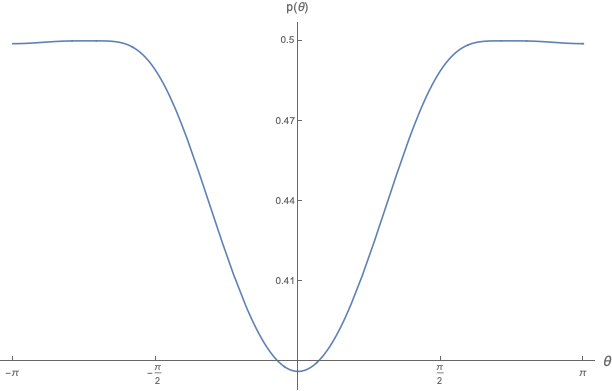
\includegraphics[width = 0.9\textwidth]{Figures/beta_1.png}
    \caption{Probability distributions of errors as a function of the position in the chain. this plot correspond to a value of $\beta=1$.}
    \label{beta1}
\end{subfigure}
\hfill
\begin{subfigure}[b]{0.45\textwidth}
    \centering
    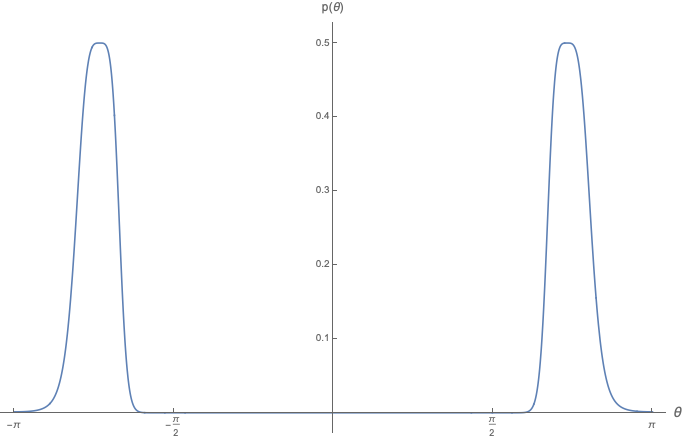
\includegraphics[width = 0.9\textwidth]{Figures/beta_80.png}
    \caption{Probability distributions of errors as a function of the position in the chain. this plot correspond to a value of $\beta=80$.}
    \label{beta80}
\end{subfigure}
\caption{An illustration of how the function $p(\theta_k)$ behaves as a function of the angle $\theta$. As we can see in both figures there are regions of the chain in which the probability of having an error is smaller.}
       \label{fig:three graphs}
\end{figure}
